\documentclass{article}
\usepackage{tikz}

\begin{document}

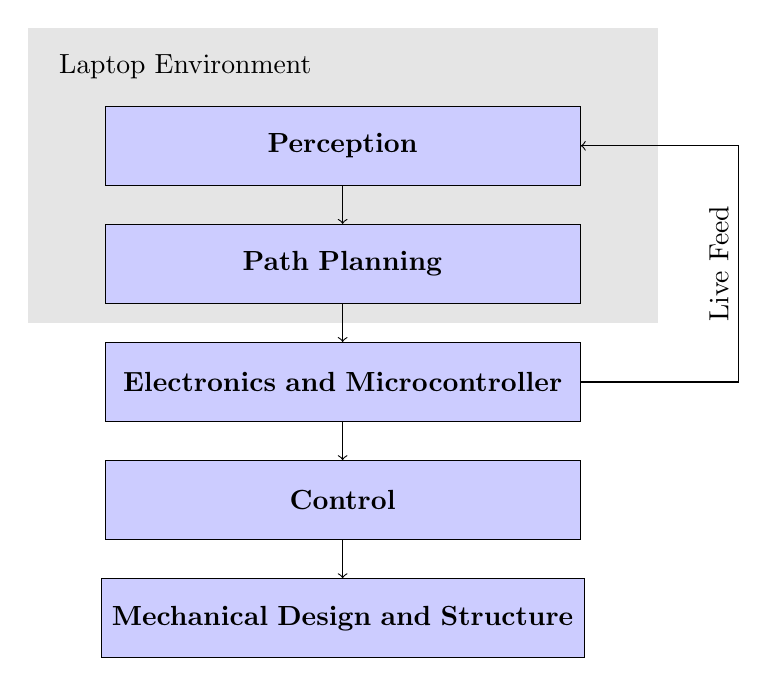
\begin{tikzpicture}
    
    % Laptop Environment
    \fill[gray!20] (-4, 1.5) rectangle (4, -2.25);
    \node at (-2, 1) {Laptop Environment};

    % Perception:
    \node[draw, fill=blue!20, minimum width=6cm, minimum height=1cm, text width=5.8cm, align=center] (Perception) at (0, 0) {
    \textbf{Perception}
    };

    % Path Planning
    \node[draw, fill=blue!20, minimum width=6cm, minimum height=1cm, text width=5.8cm, align=center] (Path Planning) at (0, -1.5) {
    \textbf{Path Planning}
    };

    % Electronics and Microcontroller
    \node[draw, fill=blue!20, minimum width=6cm, minimum height=1cm, text width=5.8cm, align=center] (Electronics) at (0, -3) {
    \textbf{Electronics and Microcontroller}
    };

    % Control:
    \node[draw, fill=blue!20, minimum width=6cm, minimum height=1cm, text width=5.8cm, align=center] (Control) at (0, -4.5) {
    \textbf{Control}
    };

    % Mechanical Design and Structure
    \node[draw, fill=blue!20, minimum width=6cm, minimum height=1cm, text width=5.9cm, align=center] (Mechanical) at (0, -6) {
    \textbf{Mechanical Design and Structure}
    };

    % Connections
    \draw[->] (Perception.south) -- (Path Planning.north);
    \draw[->] (Path Planning) -- (Electronics);
    \draw[->] (Electronics) -- (Control);
    \draw[->] (Control) -- (Mechanical);
    \draw[->] (Electronics.east) -- ++(2cm, 0) |- (Perception.east)node[pos=0.25, above, rotate=90] {Live Feed};

\end{tikzpicture}

\end{document}